\chapter{Git Collaborations}
\label{cha:git_collaboration}
This chapter contains every git command that is related to working on and with remote repositories. Thus, every command in this chapter requires a network connection to work. After finishing this chapter, the reader will be able to clone a remote repository, fetch all the existing branches and commits of that remote repository, pull additional commits from the remote repository and push new commits to the remote repository.

\newpage

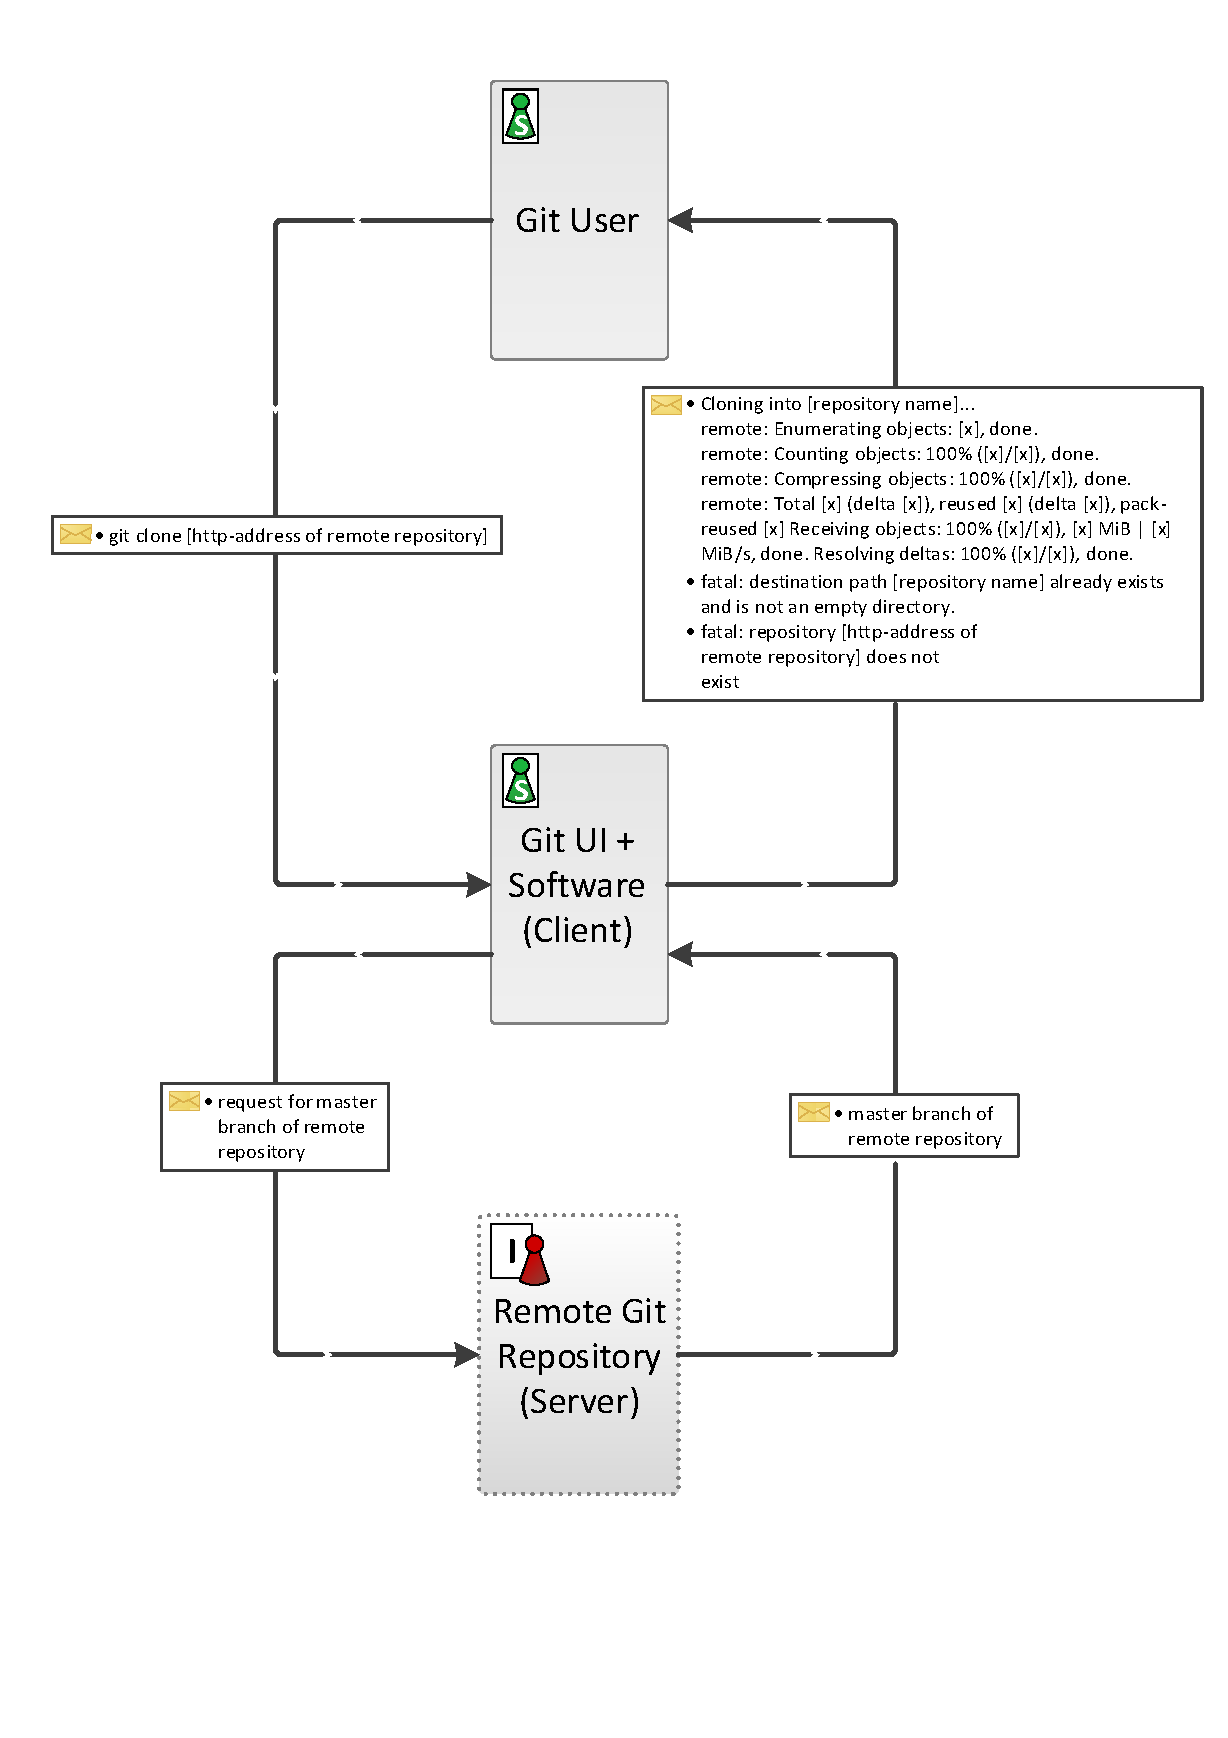
\includepdf[pages=1,pagecommand= {\section{git clone} \label{sec:git_clone}},scale=0.72]{git_commands/git_clone.pdf}
\includepdf[pages=2-last,pagecommand={} ,scale=0.75]{git_commands/git_clone.pdf}

\newpage

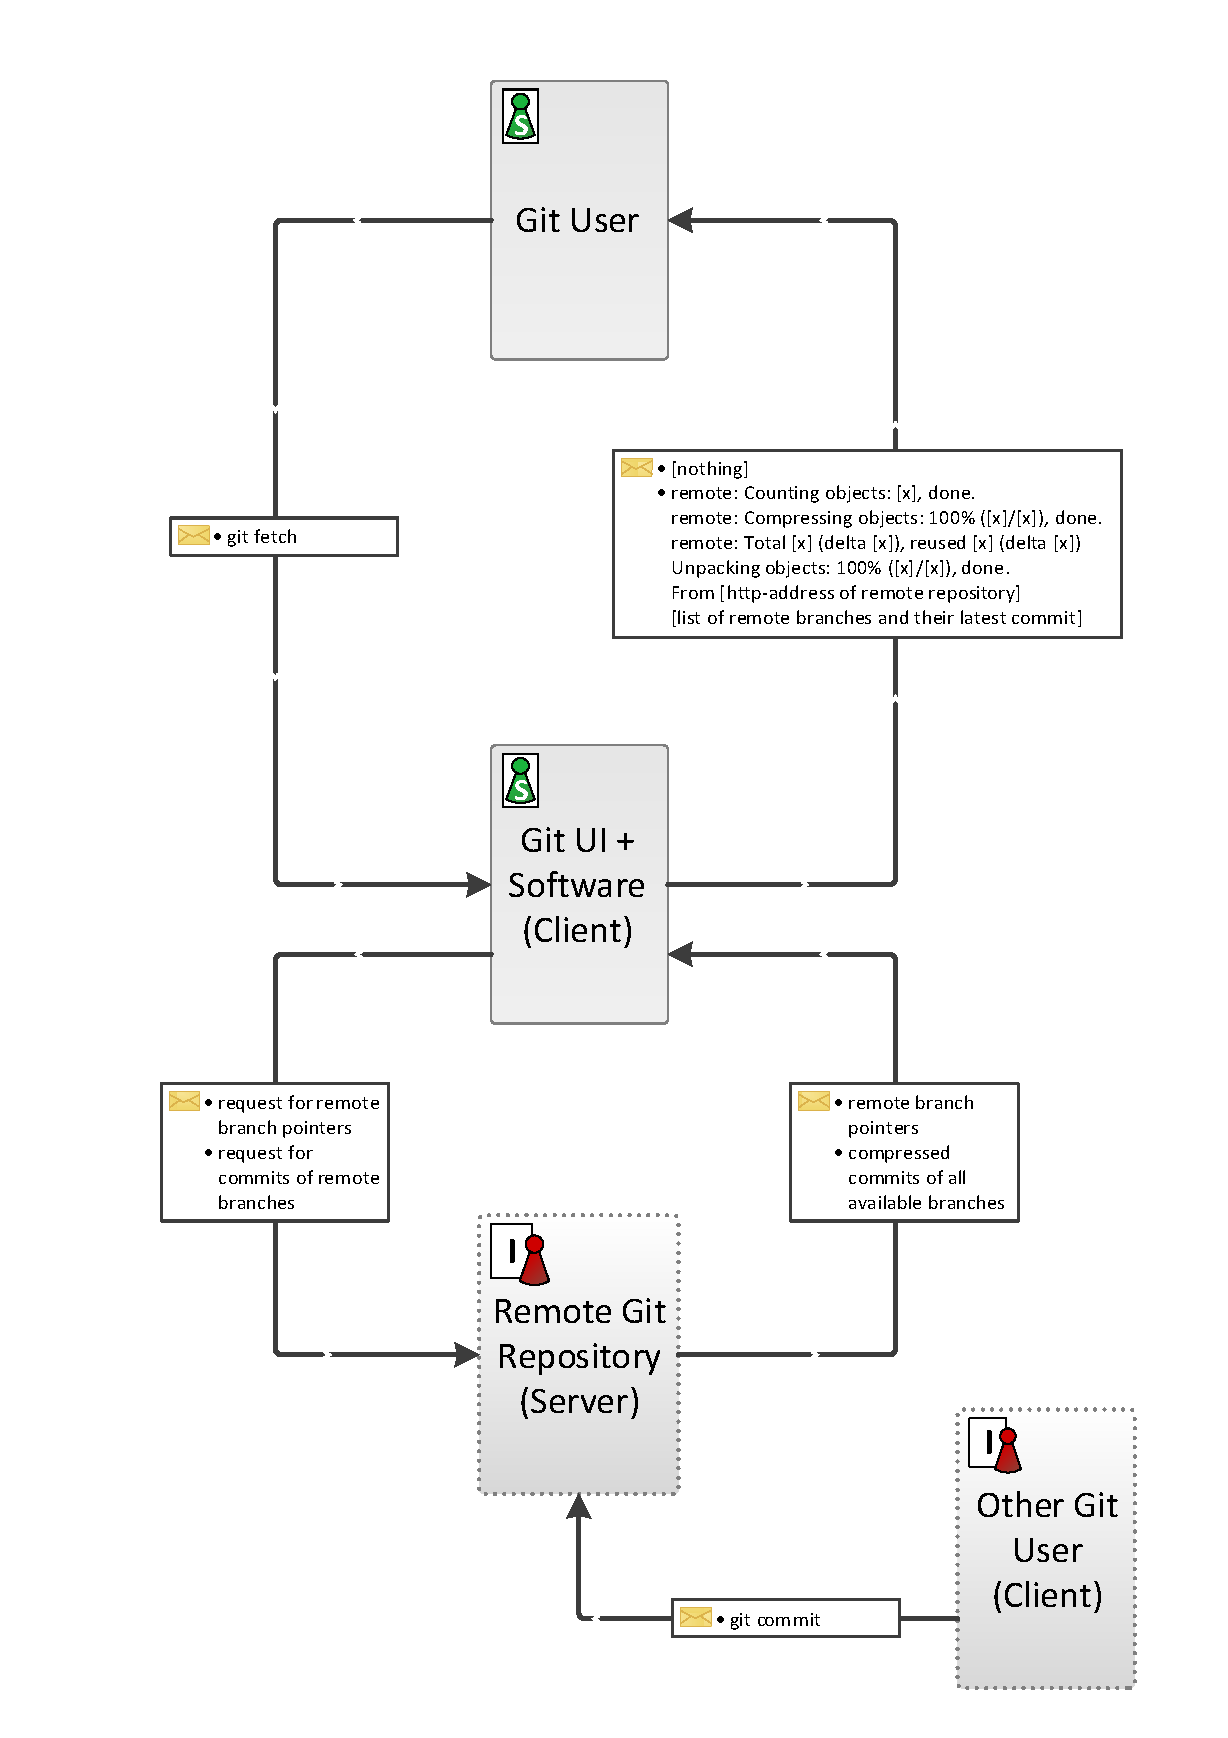
\includepdf[pages=1,pagecommand= {\section{git fetch} \label{sec:git_fetch}},scale=0.72]{git_commands/git_fetch.pdf}
\includepdf[pages=2-last,pagecommand={} ,scale=0.75]{git_commands/git_fetch.pdf}

\newpage

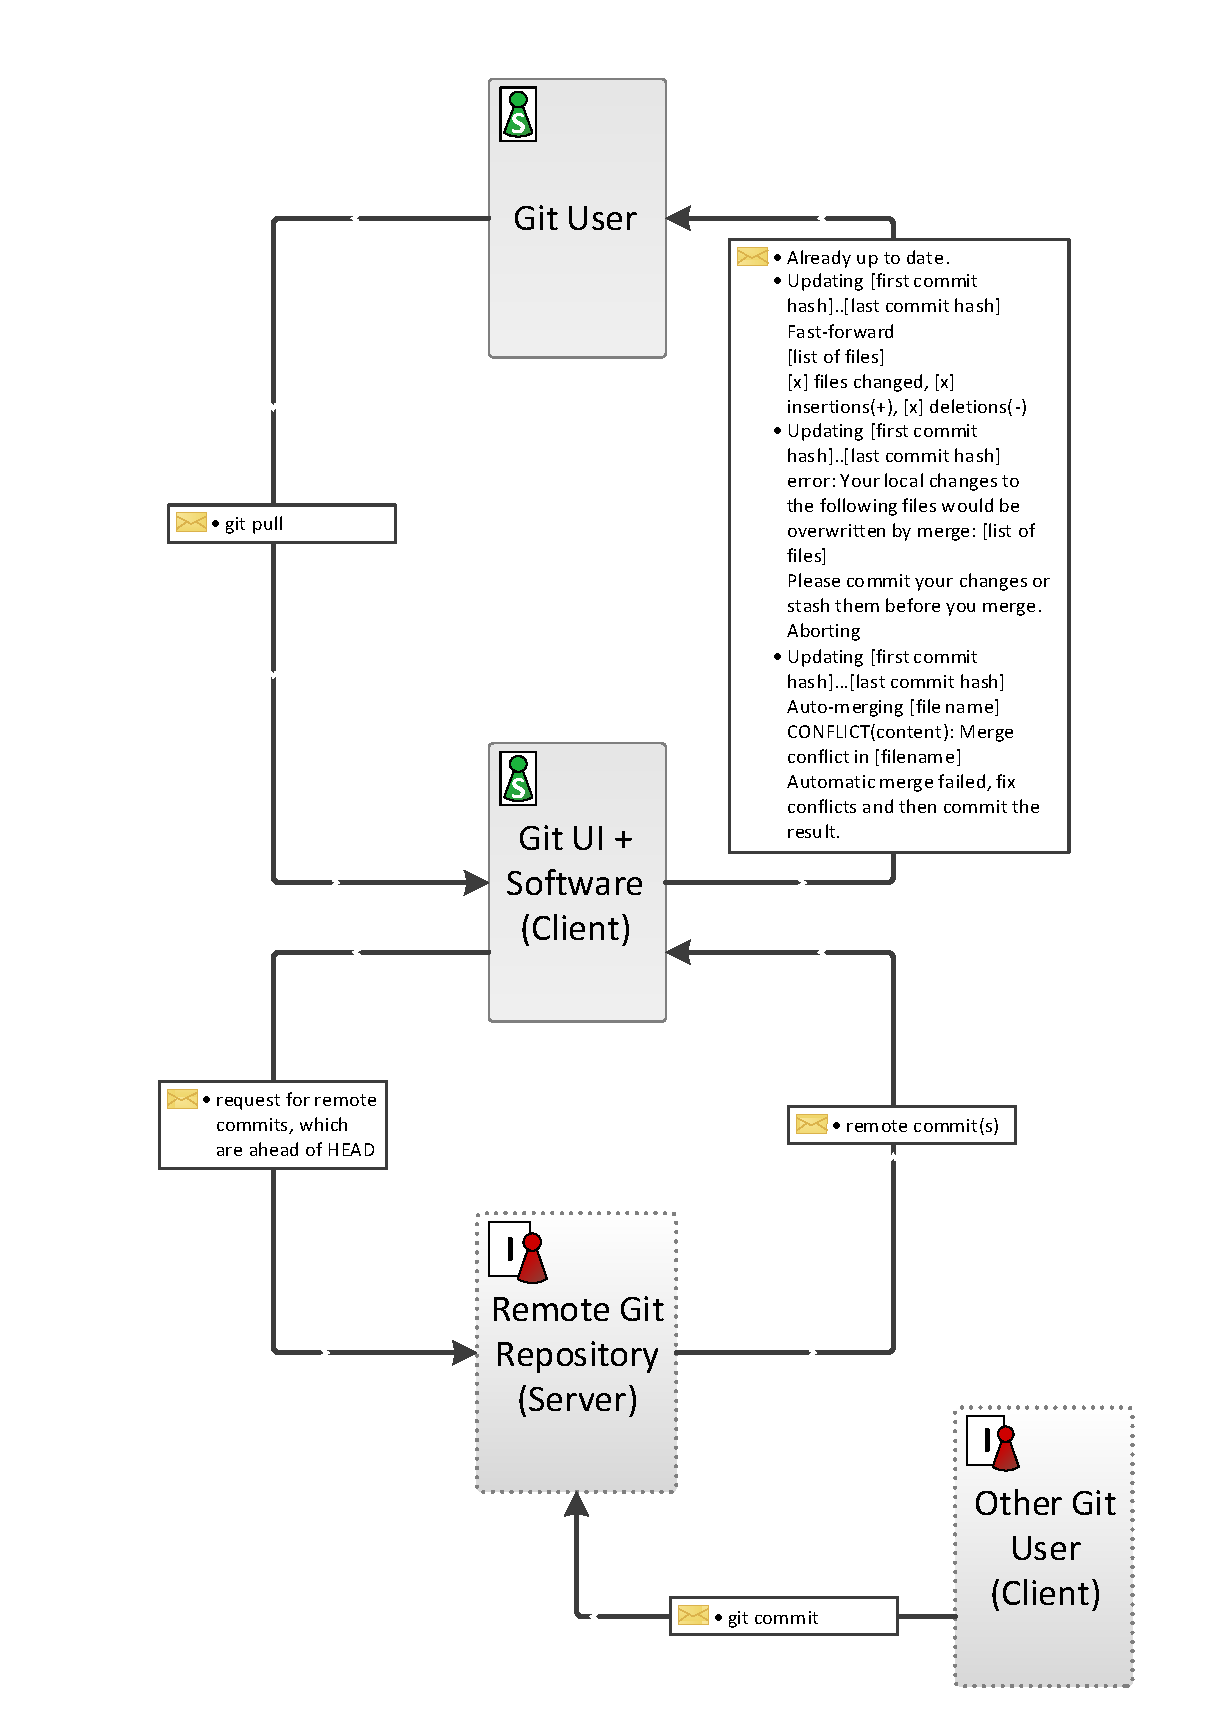
\includepdf[pages=1,pagecommand= {\section{git pull} \label{sec:git_pull}} ,scale=0.72]{git_commands/git_pull.pdf}
\includepdf[pages=2-last,pagecommand={} ,scale=0.75]{git_commands/git_pull.pdf}

\newpage

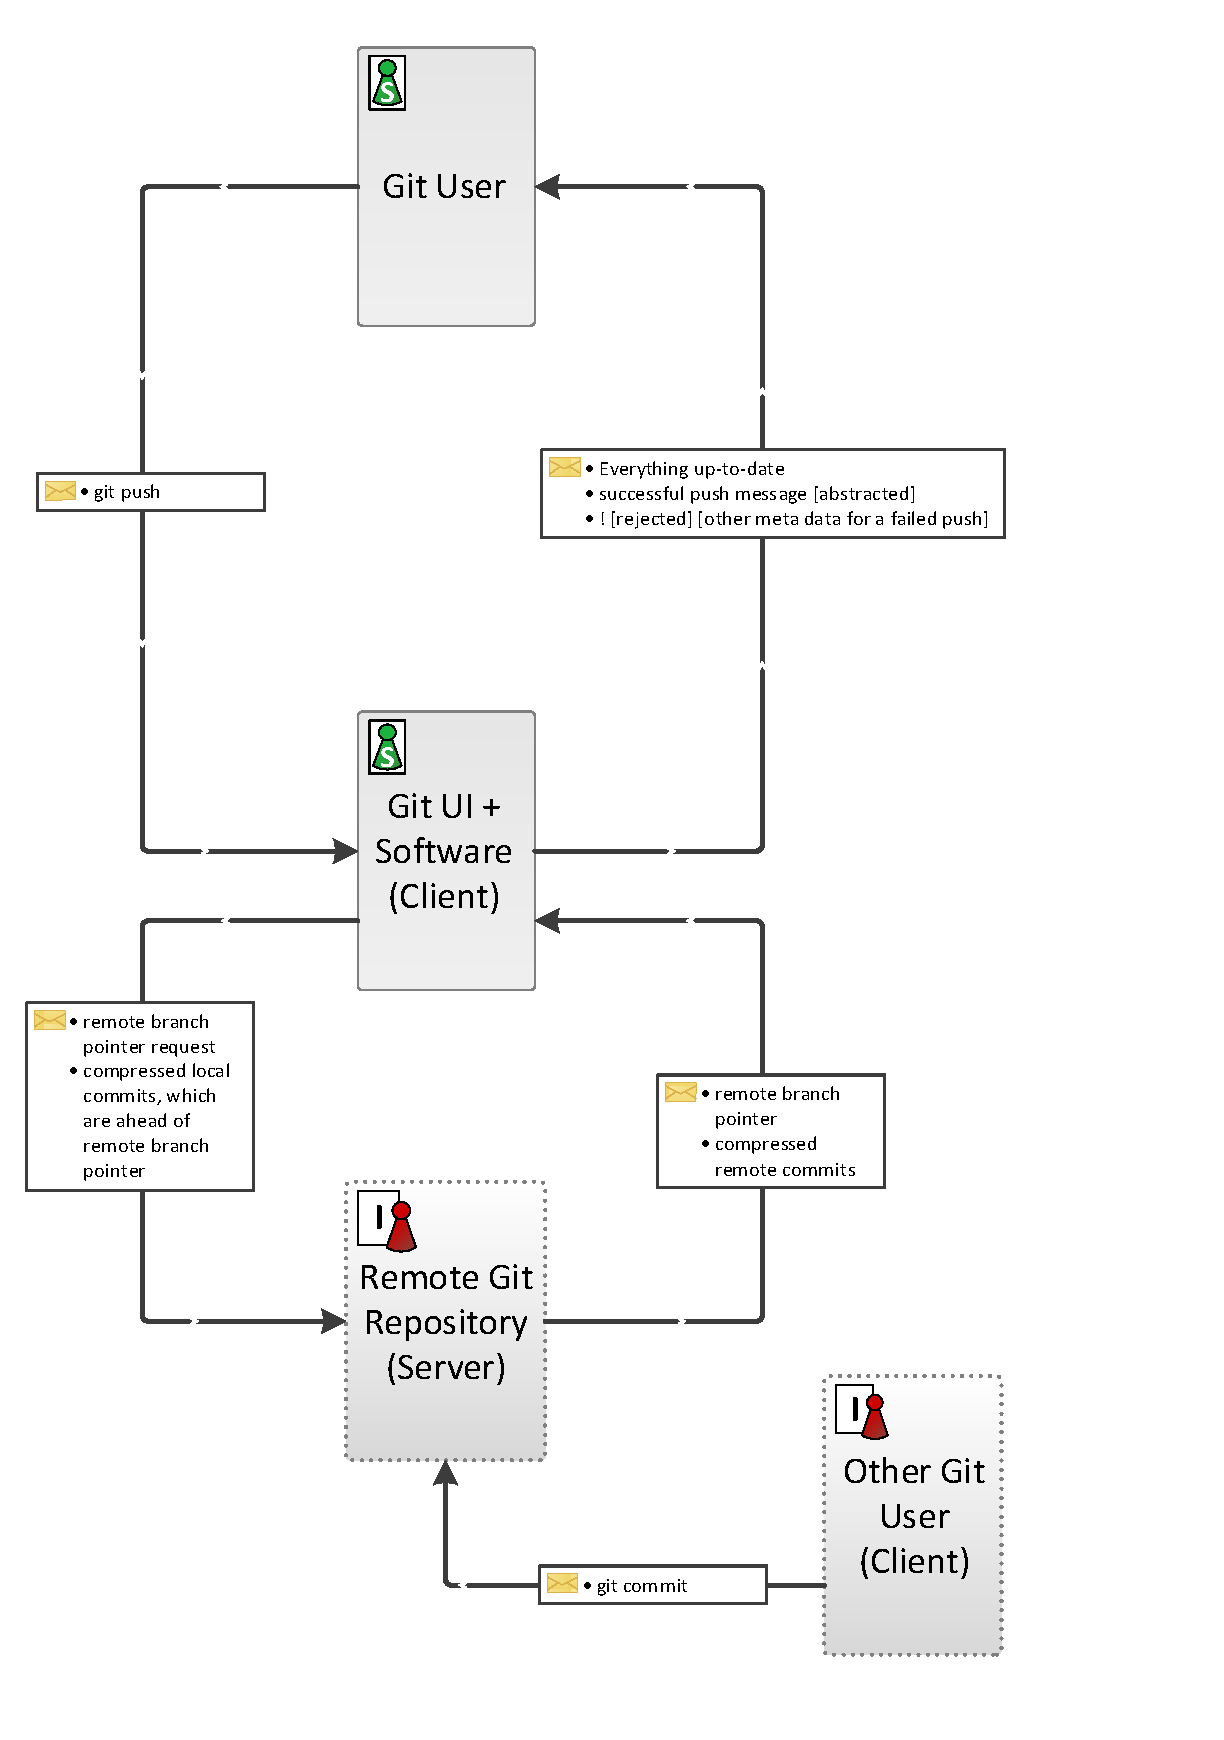
\includepdf[pages=1,pagecommand= {\section{git push} \label{sec:git_push}} ,scale=0.72]{git_commands/git_push.pdf}
\includepdf[pages=2-last,pagecommand={} ,scale=0.8]{git_commands/git_push.pdf}